% WWW 2027 Research Track submission format: anonymous double-blind review.
\documentclass[sigconf,anonymous,review]{acmart}

\usepackage{amsmath,bm}
\usepackage{booktabs,multirow,tabularx,array}
\usepackage{graphicx}
\usepackage{float}
\usepackage{enumitem}

\setcopyright{none}
\settopmatter{printacmref=false,printfolios=true}
\renewcommand\footnotetextcopyrightpermission[1]{}
\acmConference[WWW '27]{The Web Conference}{May 10--14, 2027}{Dublin, Ireland}
\acmYear{2027}
\acmDOI{}
\acmISBN{}
\graphicspath{{figures/}}
\newcommand{\method}{\textsc{CoTAG-Q}}
\newcommand{\topomethod}{\textsc{CoTAG-Q-T}}
\newcommand{\promptstudent}{prompt-based student}
\newcommand{\ours}{\method}

%!TEX root = paper.tex

%--------------- TODO Commands --------------
\newcommand{\todoc}[2]{{\textcolor{#1}{\textbf{#2}}}}
\newcommand{\wxfgreen}[1]{\textcolor[HTML]{007806}{#1}}
\newcommand{\todored}[1]{{\todoc{red}{\textbf{[[#1]]}}}}
\newcommand{\todogreen}[1]{\todoc{green}{\textbf{[[#1]]}}}
\newcommand{\todoblue}[1]{\todoc{blue}{\textbf{[[#1]]}}}
\newcommand{\todoorange}[1]{\todoc{orange}{\textbf{[[#1]]}}}
\newcommand{\todobrown}[1]{\todoc{brown}{\textbf{[[#1]]}}}
\newcommand{\todogray}[1]{\todoc{gray}{\textbf{[[#1]]}}}
\newcommand{\todopink}[1]{\todoc{pink}{\textbf{[[#1]]}}}
\newcommand{\todopurple}[1]{\todoc{purple}{\textbf{[[#1]]}}}
\newcommand{\todo}[1]{\todored{TODO: #1}}
\newcommand{\TODO}[1]{\todored{TODO: #1}}
\newcommand{\update}[1]{\todopurple{#1}}

\newcommand{\xrightarrowpad}[2][4pt]{%
  \xrightarrow{\hspace{#1}#2\hspace{#1}}%
}

%% To disable colored comments, just uncomment this line: 
%\renewcommand{\todoc}[2]{\relax}

%----------- Comment command for each person ------------
\newcommand{\xf}[1]{\wxfgreen{#1}}

% \newcommand{\eg}[0]{\textit{e.g.}}
% \newcommand{\ie}[0]{\textit{i.e.}}
\newcommand{\eg}[0]{e.g.}
\newcommand{\ie}[0]{i.e.}

\newcounter{finding}
\newcommand{\finding}[1]{\refstepcounter{finding}
    \vspace{0.5mm}
    \begin{mdframed}[linecolor=gray,roundcorner=12pt,backgroundcolor=gray!15,linewidth=3pt,innerleftmargin=2pt, leftmargin=0cm,rightmargin=0cm,topline=false,bottomline=false,rightline = false]
    \textbf{Finding \arabic{finding}:} #1
    \end{mdframed}
    \vspace{0.5mm}
}


% Keep appendix floats from triggering the final-page column balancer.
\makeatletter
\@ACM@balancefalse
\makeatother

\title{CoTAG-Q: Shared Graph and Text Support for Continual Text-Attributed Graph Condensation}
\author{Anonymous Authors}

\begin{document}
\begin{abstract}
Web content networks evolve as documents, products, and relations arrive,
while earlier training snapshots may no longer be available for model
updates. We study continual condensation of text-attributed graphs under
this access constraint. Each stage must convert the current graph into a
small memory that remains useful after release and contains readable text
for later encoding. CoTAG-Q learns a class-constrained support matrix that
coordinates graph-aware feature aggregation with the selection of a real
text source. A straight-through text interface uses the selected text in
the forward construction and a soft representation to provide optimization
feedback. Under a fixed 5\% condensation rate and a common finite student
budget, the largest matched gain is 3.47 Macro-F1 points, or 7.7\% relative,
on BookHis, with positive differences in all nine order and construction
seed combinations. The same memories retain 98.23\% and 103.33\% of the
full-history Macro-F1 on SportsFit and BookHis, respectively, while reducing
student peak GPU allocation by 93.8\% and 89.5\% and student training time
by 88.4\% and 50.9\%. Chronological streams on ArXiv, ACM, and DBLP show
that the interface also handles recurring classes, although the relative
benefit depends on the arrival stream and available graph context. The
results identify when shared graph and text support is useful and separate
downstream reuse gains from the remaining cost of memory construction.
\footnote{Data and code can be found at \url{https://anonymous.4open.science/status/www-C343}.}
\end{abstract}

\ccsdesc[500]{Computing methodologies~Learning latent representations}
\ccsdesc[300]{Information systems~Data stream mining}

\keywords{Text-attributed graphs, continual learning, graph condensation,
multimodal memory, differentiable assignment}

\maketitle

\section{Introduction}
Text-attributed graphs (TAGs) associate graph relations with text
at each node and arise naturally in Web content networks. Examples
include academic citation networks, product and purchase networks,
online knowledge communities, and linked document collections. In these
networks, graph structure supplies relational context, while node text such
as titles, descriptions, or posts supplies semantics that topology alone
cannot express. The networks are continuously updated as new content,
relations, and sometimes new classes arrive. Retraining on the accumulated
graph can preserve historical information, but its storage and training cost
grow with the entire history.

Graph condensation replaces a large training graph with a much smaller set of
training items. In the continual setting, each arriving increment must be
converted into useful memory before its raw data leaves the access
window. A later stage may receive only the current increment and the memory
written by earlier stages. For TAGs, every retained item must also carry a
readable text. The memory is therefore not merely a smaller training
set. It is the interface through which released graph and text information is
carried to future stages.

\noindent\textbf{Research gap.}
Existing studies provide complementary pieces of this problem. Static TAG
condensation uses a fully available source graph to construct compact data
that combines graph and text information~\cite{tagsam,stad}, while continual graph condensation
studies how to preserve graph training utility under a limited replay
budget~\cite{cat,puma,gecc}. Federated and multimodal condensation methods
consider related settings with different access boundaries~\cite{dance,srgm},
and graph and language alignment methods target transferable TAG prediction
rather than continual memory construction~\cite{graphclip}. These lines of
work do not explicitly define an interface in which the current graph is
converted into a compact memory before release and new memory rows are added
over time. Each retained row must preserve graph information and readable
text. This paper studies continual TAG condensation with limited access to
historical raw data.

\noindent\textbf{Two challenges.}
The access boundary and the requirement to retain text create two coupled challenges,
visualized in~\autoref{fig:challenge_overview}.

\emph{(i) Preserving graph information after source data become unavailable.}
Neighborhood information is produced from the current graph and cannot be
recovered from an isolated node feature or text string after the raw
increment is released. Later stages cannot recompute the released
neighborhoods or jointly recondense those nodes with future data. The
constructor must therefore decide what relational evidence to commit to a
small memory while classes and graph patterns continue to change. The
memory must carry this information into later stages. This makes the
balance between preserving earlier knowledge and learning new information
central to continual condensation.

\emph{(ii) Coordinating continuous feature construction with discrete text selection.}
Condensation combines information from multiple nodes, but the stored text
must be a real and readable source string. A continuous pooled representation
need not correspond to an actual string. Selecting text only after feature optimization can
break the correspondence between a synthetic feature and its text, whereas
storing an optimized text vector loses provenance and auditability. A
continual TAG condenser must coordinate feature construction and text
selection so that the retained features and readable texts describe
compatible source information.

\begin{figure}[t]
\centering
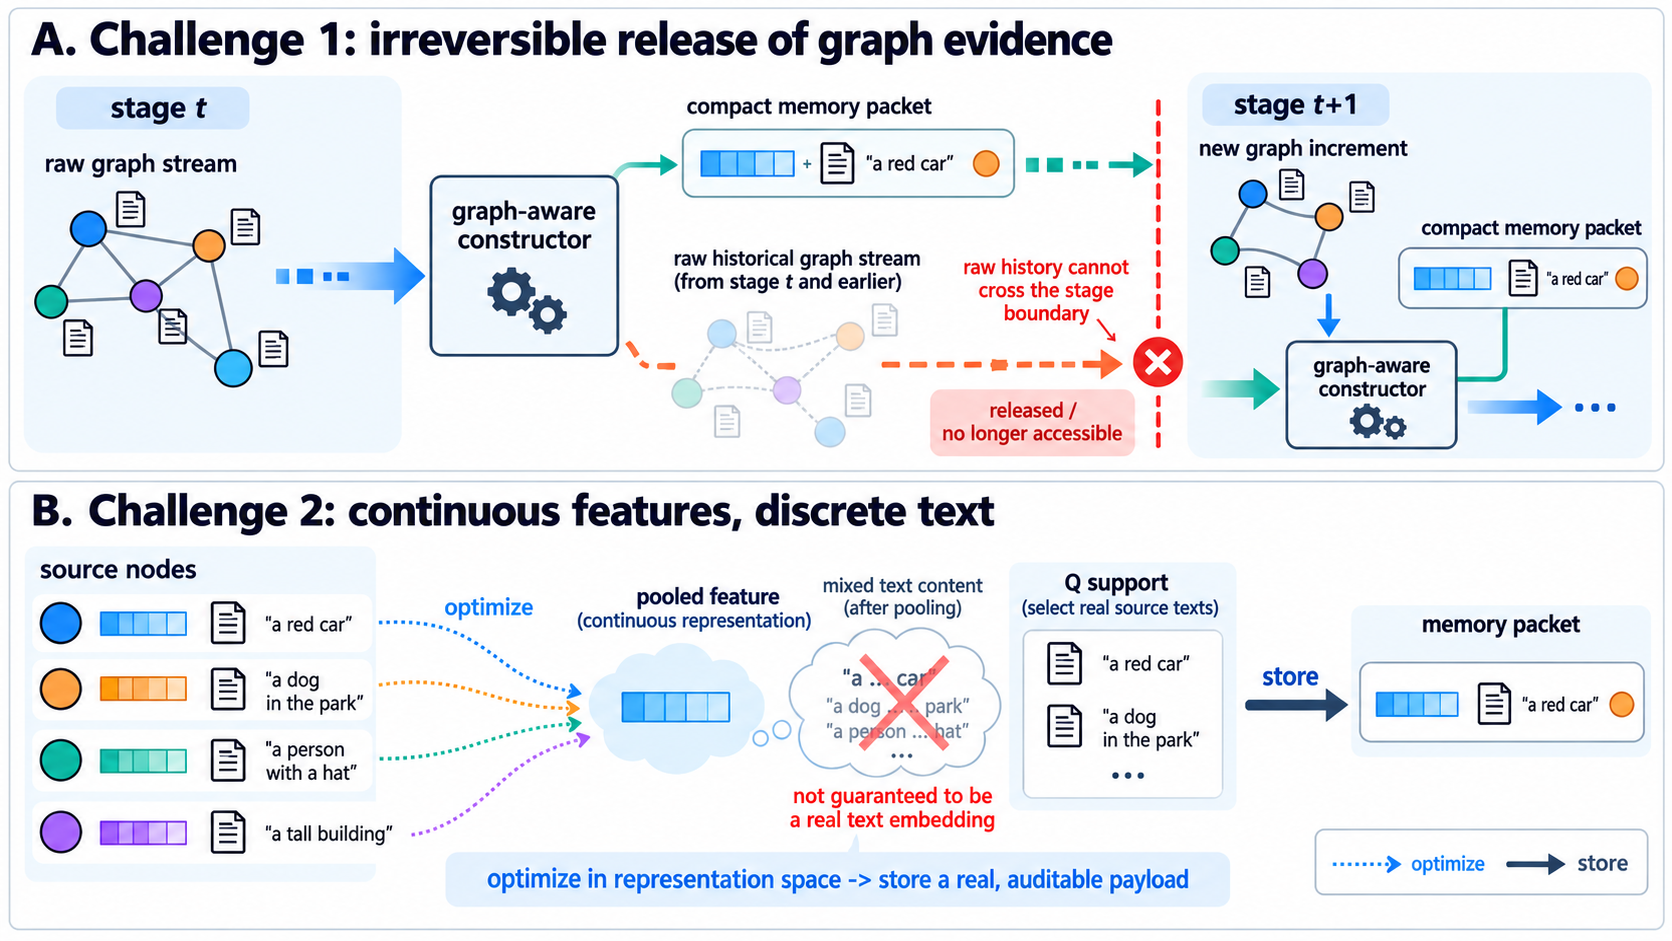
\includegraphics[width=\columnwidth]{challenge_overview_v2.png}
\caption{Information flow in the two challenges. Only the compact memory
crosses the stage boundary after the raw increment is released. The
lower panel shows the conversion from continuous feature construction to a
real, auditable text.}
\Description{Two compact panels visualize irreversible release of a raw graph
increment and the mismatch between continuous feature construction and
discrete text selection.}
\label{fig:challenge_overview}
\end{figure}

\noindent\textbf{Design principles and CoTAG-Q.}
The two challenges motivate three design principles. Graph information
should be extracted before release. Feature construction and text selection
should use one auditable support matrix. The text rule used during
construction should also agree with the text that is ultimately stored.

We propose \method{} around these principles. At each stage, the current
graph is used to construct new memory items, historical memory
is kept fixed, and only new items are appended. A support matrix constrained
by class labels coordinates feature aggregation with text selection.
Neighborhood summaries guide numerical features, and training feedback
refines the source contributions used by both features and text.
Algorithmic details are given in~\autoref{sec:method_interface}.

Under a fixed condensation rate, \method{} improves recognition of
historical classes on BookHis and retains high training utility relative
to all observed raw data on the two product graphs. The same memories
also train a GraphSAGE student without further construction. Chronological
streams extend the evaluation to document arrivals with recurring classes.
Training on the condensed memory also reduces the cost of subsequent student
updates, while construction remains a separate upfront cost.
The experiments report the detailed comparisons, robustness checks, and
limitations of these results.

\noindent\textbf{Contributions.}
\begin{itemize}[leftmargin=*,nosep]
\item We formulate continual TAG condensation with an explicit historical
access boundary. Each stage receives the current increment and a stored
condensed memory. Each retained item contains numerical features that
preserve graph information together with readable text.
\item We propose \method{}, which learns a support matrix constrained by
class labels for feature aggregation and text selection
before the current source is released.
\item We establish a consistent construction and storage interface for readable
text and evaluate memory retention, architecture transfer, construction cost,
and a separate topology extension under the same continual protocol. We also
measure downstream reuse: under a common student budget, condensed memories
reduce peak GPU allocation by 89.5--93.8\% and training time by 50.9--88.4\%
relative to the full observed training pool.
\end{itemize}


\section{Problem Setting and Evaluation Protocol}
\label{sec:protocol}
We define the graph stream and its access constraints, specify the condensed
memory and its allocation, and then describe how memory utility is evaluated.

\subsection{Graph Stream and Historical Access}
\label{sec:stream_setting}

Citation networks and Web product catalogs receive new documents or products
in successive batches. Storage costs and data retention policies can limit
access to earlier records for model updates. We model this situation by
allowing construction access to each raw batch for a limited period, during
which useful training information must be retained in a smaller memory.

The stream has $T$ stages. The \emph{current increment} at stage $t$ is
$\Delta_t=(V_t,X_t,T_t,Y_t,E_t)$. Here $V_t$ contains the $n_t=|V_t|$
\emph{construction nodes}, $X_t\in\mathbb R^{n_t\times d_x}$ contains their
$d_x$-dimensional features, $T_t=\{t_i:i\in V_t\}$ contains their texts,
and $Y_t=\{y_i:i\in V_t\}$ contains their available labels. The edges
$E_t\subseteq V_t\times V_t$ are induced on these nodes, with adjacency
$A_t\in\{0,1\}^{n_t\times n_t}$. Neighborhood information used in
construction comes from the current increment. Held-out nodes are excluded from this input so their
features and texts cannot serve as construction examples.

Let $\mathcal C_t$ denote the classes present in the current increment, and let
$\mathcal C_{\leq t}=\bigcup_{\tau=1}^t\mathcal C_\tau$ denote all
classes observed so far. Our primary evaluation uses class-incremental streams,
following continual graph condensation studies~\cite{cat,puma}. Their class sets
are disjoint, and a \emph{class order} determines which classes enter each stage.
This partition tests retention as the label space expands. We also evaluate
chronological streams, in which publication year determines arrival and
classes may recur across stages. \autoref{sec:setup} gives both schedules.

At stage $t$, the constructor receives $\Delta_t$ and the
\emph{historical memory} $M_{t-1}$. Once the new memory is saved, the raw
nodes, texts, features, and edges of $\Delta_t$ are unavailable to later
construction stages. Memory therefore carries earlier information into later
construction. The goal is to retain training information for predicting all
observed classes using this compact memory. Downstream graph access is
specified separately below.

\subsection{Condensed Memory and Fixed Condensation Rate}
\label{sec:memory_setting}

A \emph{memory item} contains a numerical feature, readable text, and a
class label. A \emph{memory slot} is the position allocated to an item
before its feature and text are constructed. The new block is
$M_t^+=\{(x_j^+,t_j^+,y_j)\}_{j=1}^{m_t}$, where $m_t$ is the number of
new slots and superscript $+$ denotes the new block. Starting from
$M_0=\varnothing$, the constructor $\mathcal F_t$ at stage $t$ produces
\begin{equation}
 M_t=M_{t-1}\oplus M_t^+,
 \qquad M_t^+=\mathcal F_t(\Delta_t,M_{t-1}),
\label{eq:continual_memory}
\end{equation}
where $\oplus$ appends the new items. Historical memory remains fixed
during this operation. This design preserves previously constructed features
and texts when their sources are unavailable, and separates construction of
new items from historical revision. We use this fixed access policy
throughout the experiments.

The \emph{fixed condensation rate} $\rho\in(0,1]$ controls the number of retained
items relative to the number of observed construction nodes. With
$N_t=\sum_{\tau=1}^{t}n_\tau$, the nominal capacity is
$\bar K_t=\operatorname{round}(\rho N_t)$. We reserve at least one new
slot for each class in $\mathcal C_t$, giving actual capacity
$K_t=\max\{\bar K_t,|M_{t-1}|+|\mathcal C_t|\}$ and
$m_t=K_t-|M_{t-1}|$. Remaining slots use largest-remainder rounding,
subject to the number of available nodes in each class. This prevents
integer rounding from excluding a class in the current increment. We report the
effective rate $K_t/N_t$ when this coverage requirement changes the nominal
rate. Following graph condensation with a fixed rate~\cite{cat}, the allocation
keeps compression comparable as data accumulates. Memory
size grows with the stream. The rate constrains the number of retained
nodes rather than bytes or GPU memory. Its numerical value and
sensitivity study are given with the experiments.

For \method{}, the \emph{support matrix}
$Q\in\mathbb R_{\geq0}^{n_t\times m_t}$ links current nodes to new slots.
Its learnable scores are $Z\in\mathbb R^{n_t\times m_t}$, and
$R\in\mathbb R^{m_t\times d_x}$ denotes the feature residual added to
the pooled features. Text $\bar t_i$ denotes the cleaned source string,
and $e_i\in\mathbb R^{d_e}$ its normalized embedding, where $d_e$ is the
text encoder's output dimension. \emph{Hard text selection} chooses a
source string for a slot. A \emph{soft text representation} is a weighted embedding mixture
used to supply gradients. \emph{Materialization} means saving the final
features, selected strings, labels, and source identifiers. The main
memory is \emph{edge-free}, storing feature and text items without edges
between them while incorporating graph context during construction.
\autoref{sec:method_interface} explains the
corresponding computations.

\subsection{Downstream Learning and Evaluation}
\label{sec:evaluation_protocol}

The \emph{student model} is the downstream predictor trained on condensed
memory using graph and text pairing and class prompt supervision. A \emph{class prompt} is a
predefined text description of a label. Prediction at stage $t$ compares a
node's graph representation
$h_i^g$ with the projected, normalized prompt representation $p_c$ for
$c\in\mathcal C_{\leq t}$, selecting the largest cosine similarity. This
readout with class prompts evaluates whether memory supports graph and language
alignment~\cite{graphclip}. Construction and training use class labels,
so the task is supervised classification of observed classes. A
\emph{proxy model} supplies a training signal during memory construction.

Evaluation is transductive. The student model can use the original graph
structure and node features at inference, while evaluation labels are
withheld from construction and training. An \emph{evaluation mask}
specifies which nodes are scored. Matched comparisons use common text
processing, encoders, class prompts, memory allocation, class orders,
student models, and downstream training budgets. The implementation,
metrics, and repetition statistics are specified in~\autoref{sec:setup}.


\section{Related Work}
\noindent\textbf{Text-attributed graph learning.}
TAGs encode node semantics through text and relations through edges. Existing
benchmarks compare language models, graph neural networks, and their joint
training~\cite{tag_benchmark}. Common graph encoders include convolution,
attention, message passing, and inductive neighborhood aggregation
~\cite{gcn,gat,mpnn,graphsage,gin}. Earlier network representation methods
use random-walk neighborhoods to obtain compact node features
~\cite{deepwalk,node2vec}, while text encoders and multimodal
alignment models provide semantic representations~\cite{bert,sbert,clip}.
GraphCLIP learns transferable representations by contrasting graphs with text
summaries~\cite{graphclip}, and graph self-supervision provides related ways
to improve representation quality~\cite{dgi,graphcl}. Continual adaptation
coordinates modality updates to mitigate forgetting~\cite{g2lora}. These
studies focus on learning and adapting models. We study the training data
retained between updates, constructing compact memories that contain both
numerical features and real text for subsequent encoding.

\noindent\textbf{Graph condensation.}
Dataset condensation has used gradient matching, distribution matching, and
training-trajectory matching to preserve the behavior of a larger training
set~\cite{dataset_gradient,dataset_distribution,trajectory_matching}.
Graph condensation extends these ideas to relational data~\cite{gcond,sfgc}
and has developed benchmarks, inductive node mappings, and open-world
settings~\cite{gcondenser,mcond,opengc}. Structure can guide feature
construction even when the resulting training set stores no synthetic edges.
Our setting additionally requires readable text for every memory item. The
learned support matrix coordinates the contribution of current nodes to
numerical features and the selection of a real text source, giving these two
components a common construction variable.

\noindent\textbf{TAG and multimodal graph condensation.}
TAGSAM combines subgraph text selection with attribute matching~\cite{tagsam}. STAD combines cluster compression with text generation~\cite{stad}, and TaLK optimizes continuous token embeddings~\cite{talk}. DANCE uses training feedback for dynamic neighborhood and text selection in federated learning~\cite{dance}. SR-GM addresses modality conflicts through gradient decoupling and structural regularization~\cite{srgm}. These methods establish several ways to couple text and graph compression. Our focus is constructing successive memory increments after earlier raw data become unavailable. Within each increment, real text selection receives surrogate gradients through the support used for feature aggregation, while historical memory supplies context for the construction objective.

\noindent\textbf{Continual graph learning and evolving condensation.}
Continual learning studies how to preserve earlier knowledge while new data
arrive, using replay, parameter regularization, or distillation
~\cite{icarl,ewc,lwf,continual_survey}. Dynamic graph models instead update
representations as nodes, attributes, and edges evolve~\cite{evolvegcn,tgn,
dynamic_survey}. Class-incremental graph learning also exposes the tension
between retaining earlier classes and adapting to new ones~\cite{qi2024}.
In graph condensation, replay methods address historical
coverage and class representativeness~\cite{dslr}, CaT reduces the imbalance
between incoming data and replay through condensation and training in memory
~\cite{cat}, PUMA incorporates unlabeled information and reduces repeated
propagation and condensation costs~\cite{puma}, and GECC inherits clustering
states of aggregated features for evolving condensation~\cite{gecc}. These
approaches motivate a compact state that can persist across updates. We extend
that interface to paired numerical features and readable text, constructing
new items from the current increment and historical memory. This addresses
the additional information that a graph and text learner requires after the
original increment is released.


\section{Learning Graph and Text Support}
\subsection{Method Overview}
\label{sec:method_interface}

\method{} constructs compact training memories that carry graph information
and readable text across stages. This requires preserving relational
context before the current graph is released and coordinating numerical
feature construction with discrete text selection. We address these two
challenges through a learnable support matrix $Q$, where $Q_{ij}$ measures
the contribution of current node $i$ to new memory slot $j$. Each column
defines the source nodes from which a feature and its associated text are
constructed.

\autoref{fig:method_flow} summarizes three connected components.
\emph{Support learning} combines node features, neighborhood information,
and text semantics to initialize and refine $Q$
(\autoref{sec:method_support}).
\emph{Joint construction} converts this support into numerical features
and real texts, with a differentiable path for text feedback
(\autoref{sec:method_payload}).
\emph{Optimization and continual update} match the candidate memory to
current graph evidence and training signals, then append the resulting
block to the accumulated memory (\autoref{sec:method_update}).
Together, these components transfer current graph information into memory
features and allow training feedback from the selected texts to influence
their construction.

\begin{figure*}[t]
\centering
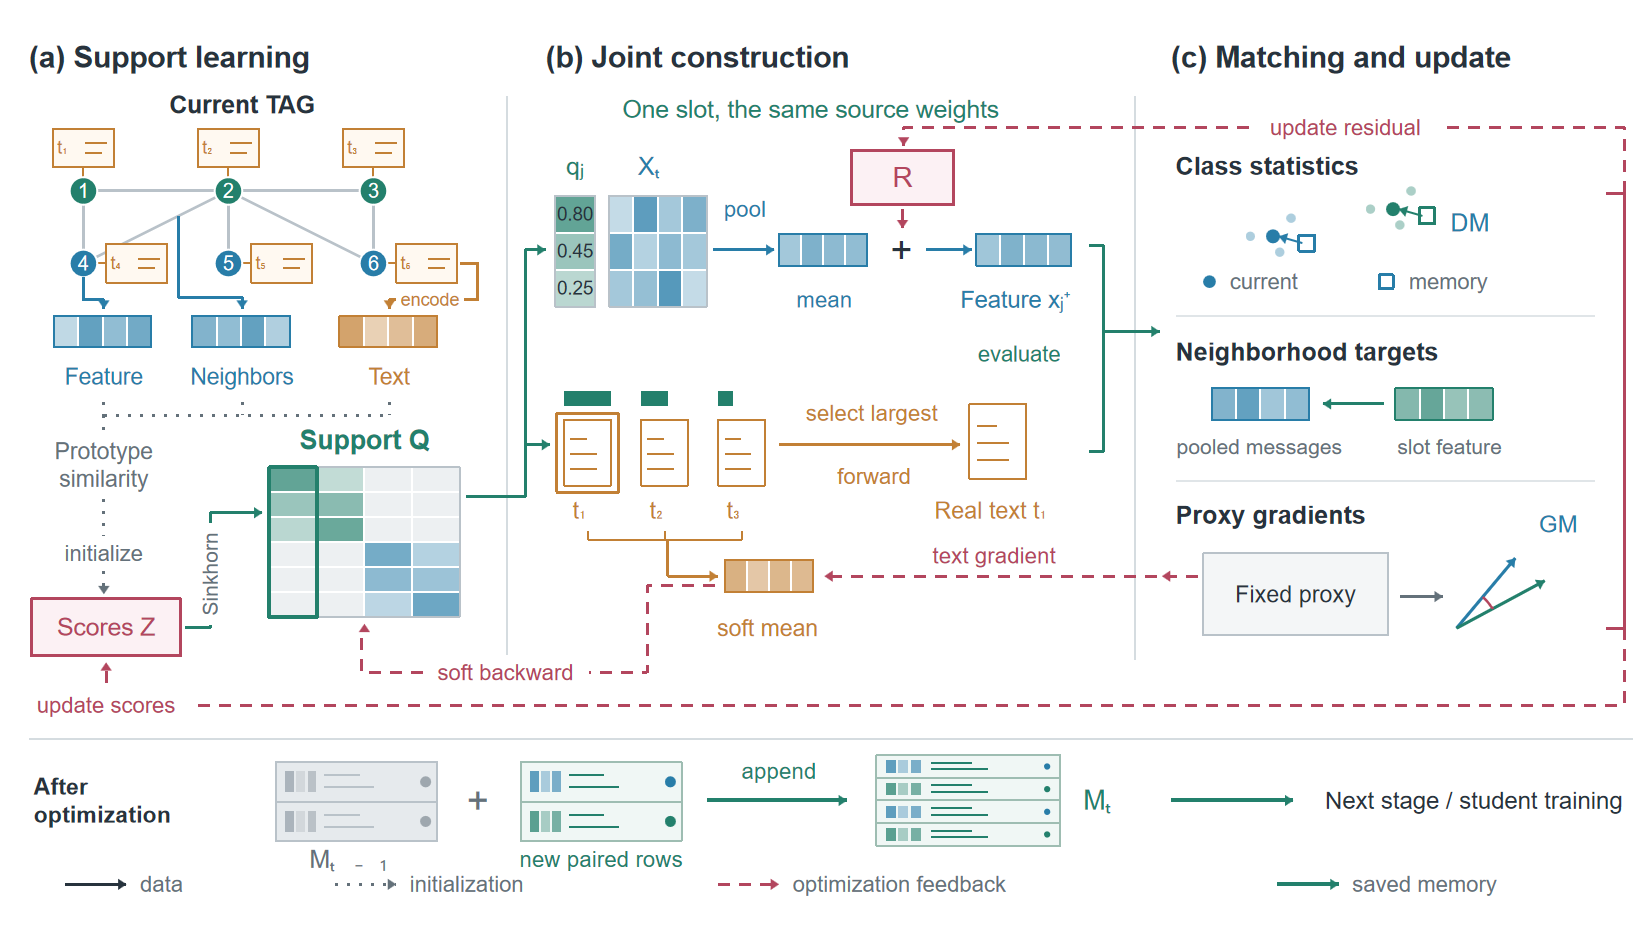
\includegraphics[width=\textwidth]{method_overview_final.png}
\caption{Overview of \method{}. (a) Node features, neighborhood context,
and attached texts from the current TAG initialize a balanced support matrix. (b) One slot and its
sources of the same class illustrate feature aggregation and real text selection
under $Q$. The soft text mean provides the backward path. (c) Class
statistics, neighborhood targets,
and proxy gradients guide construction. Proxy gradients use the same
accumulated memory on both sides. The optimized feature and text rows are
appended to memory for the next stage.}
\Description{Three panels show support learning, joint construction, and
matching. Each numbered node in the current TAG carries a corresponding text
attribute. Node features, neighborhoods, and encoded texts initialize scores.
A support matrix organized by class links nodes to slots.
One column supplies feature pooling and discrete document selection, with
a soft text representation for backpropagation. Comparisons with current
graph statistics and proxy training gradients update the support scores
and feature residual. A bottom strip shows old and new paired memory rows
being combined and passed to the next stage.}
\label{fig:method_flow}
\end{figure*}

\subsection{Learning Support from Graph and Text}
\label{sec:method_support}

The support matrix identifies which current nodes can jointly represent a
slot. Feature similarity alone describes individual attributes, whereas
neighboring nodes supply relational context and source texts supply
semantic content. We therefore describe each node using three normalized
views, comprising its numerical feature, a message aggregated from the normalized
features of its current neighbors, and the embedding of its cleaned text
from the frozen MiniLM encoder. Normalizing each view makes its similarity
depend on direction rather than vector magnitude.

At stage $t$, $Q$ has $n_t$ rows and $m_t$ columns, as defined in
\autoref{sec:memory_setting}. Within each
class, farthest-point selection on the combined representation provides
initial slot prototypes. Selecting points distant from the existing
prototypes spreads the starting slots across different regions of the
class. Let $\psi_i$ and $\pi_j$ denote the three views of node $i$ and
prototype $j$. Their initial support score is
\begin{equation}
 Z^0_{ij}=\operatorname{sim}(\psi_i,\pi_j),
 \qquad y_i=y_j .
\label{eq:method_init}
\end{equation}
Here $\operatorname{sim}$ is a weighted sum of cosine similarities of the
corresponding feature, neighborhood, and text views. The resulting
$Z^0$ initializes learnable scores $Z$. A class mask restricts each slot
to sources with its label, so the support has a block structure over
classes.

At each forward pass, we scale $Z$ by a temperature and apply Sinkhorn
normalization~\cite{sinkhorn} within each class block. Alternating row and
column normalization gives every node unit total mass and targets a mass
of $n_c/m_c$ for each slot in class $c$, where $n_c$ and $m_c$ are its
numbers of current nodes and slots. Iteration enforces these marginals
to numerical tolerance. This balancing distributes the class's support
across the available slots. Soft assignments let a source contribute to
several slots, while differentiability allows subsequent objectives to
refine those contributions. Thus, graph and text similarity provide the
starting organization, and memory construction supplies the signal for
learning it further.

\subsection{Joint Feature and Text Construction}
\label{sec:method_payload}

\textbf{Feature aggregation.}
For each slot, $Q$ defines a weighted set of source nodes. Let
$a_j=\sum_i Q_{ij}$ be its total support mass and let
$D_a=\operatorname{diag}(a_1,\ldots,a_{m_t})$. The feature branch computes
the corresponding weighted mean and adds a learnable residual,
\begin{equation}
 \bar X_t=D_a^{-1}Q^{\top}X_t,\qquad
 X_t^{+}=\bar X_t+R .
\label{eq:method_feature}
\end{equation}
Dividing by $a_j$ separates the scale of a feature from the number of
sources supporting it. Each pooled row is consequently a convex
combination of source features. The residual $R$ allows a local correction
beyond this average, which is useful when the subsequent graph and
training targets cannot be expressed by pooling alone. We initialize $R$
at zero and bound each row's norm relative to its current pooled feature
norm. The two variables have complementary roles. $Z$ changes which
sources contribute, while $R$ adjusts the resulting numerical feature.

\textbf{Text selection and feedback.}
The text branch selects the largest entry in the same column of $Q$,
giving source index $i_j^*$. The class mask ensures that the source and
slot share a label. The slot stores that source's
cleaned string $t_j^+=\bar t_{i_j^*}$. This gives the numerical mixture
and readable text a common source support. However, changing the scores
slightly may leave the selected index unchanged, preventing ordinary
backpropagation through the discrete choice. We therefore also form a
soft text mean. With $e_i$ denoting the normalized source embedding and
$\operatorname{Norm}$ denoting vector normalization, we use
\begin{equation}
\begin{aligned}
 \widetilde e_j
   &=\operatorname{Norm}\!\left(\frac{1}{a_j}\sum_i Q_{ij}e_i\right),\\
 e_j^{\mathrm{ST}}
   &=e_{i_j^*}+\widetilde e_j-\operatorname{sg}(\widetilde e_j).
\end{aligned}
\label{eq:method_text}
\end{equation}
The superscript ST denotes a straight-through estimator. The stop-gradient
operator $\operatorname{sg}$ preserves its input value
and stops its derivative. In the forward pass the soft terms cancel,
giving $e_j^{\mathrm{ST}}=e_{i_j^*}$, so the candidate is evaluated with
the real text it would store. In the backward pass the soft mean supplies
a surrogate derivative with respect to $Q$. With the text encoder fixed,
feedback changes the support scores. These changes modify
the feature mixture and can switch the selected text in a later forward
pass. In this way, text participates in construction through its training
signal as well as its initial similarity.

\subsection{Optimization and Continual Update}
\label{sec:method_objectives}
\label{sec:method_update}

The objectives guide the constructed rows through class
statistics, individual neighborhood representations, and the learning
signal of the student model.

\textbf{Retaining graph information.}
We first cache $H_t$, obtained by applying the symmetrically normalized
current adjacency with self-loops to $X_t$. Its row $h_i$ summarizes
the feature and neighborhood context of current node $i$.
For distribution matching (DM), we compare these messages with the candidate
features after nonlinear projections
$\phi_b(v)=\operatorname{Norm}(\operatorname{ReLU}(vW_b))$, where the
$B$ random matrices $W_b$ are fixed throughout construction and ReLU is the
rectified linear activation. Let $V_{t,c}$
and $S_{t,c}$ contain current nodes and new slots of class $c$,
respectively. We match their projected class means,
\begin{equation}
 L_{\mathrm{DM}}=\frac{1}{B}\sum_{b=1}^{B}\sum_{c\in\mathcal C_t}
 \left\|
 \frac{\sum_{i\in V_{t,c}}\phi_b(h_i)}{|V_{t,c}|}
 -\frac{\sum_{j\in S_{t,c}}\phi_b(x_j^+)}{|S_{t,c}|}
 \right\|_2^2 .
\label{eq:method_dm}
\end{equation}
Matching means in several nonlinear feature spaces constrains class
statistics beyond the original feature mean. Since the reference uses
propagated features, reducing this discrepancy transfers graph context
into the compact numerical representations.

Class means alone leave individual slots underconstrained. Propagation
matching therefore gives each slot a local target by pooling the rows of
$H_t$ with weights $Q_{ij}/a_j$ and normalizing the result. It penalizes
the angular discrepancy between this target and the normalized candidate
feature. The same source weights define both the feature mixture and its
neighborhood target. This term complements matching of class means by
retaining information about the
specific region represented by each slot.

\textbf{Retaining training signals.}
Feature statistics do not directly measure how a feature and its selected
text interact under the training objective. We therefore evaluate fixed
proxy models with the student's graph and text pairing loss and class
prompt supervision. For proxy $p$, let $g_p^{\mathrm{ref}}$ and
$g_p^{\mathrm{mem}}$ denote flattened parameter gradients evaluated on
the current increment and the candidate block, respectively, with
$M_{t-1}$ included on both sides. The accumulated memory thus supplies
the same historical training context for both gradients. We average
their direction and log magnitude discrepancies over $P$ proxy
initializations to define the gradient matching (GM) loss,
\begin{equation}
\begin{aligned}
 L_{\mathrm{GM}}=\frac{1}{P}\sum_{p=1}^{P}\bigg[&
 1-\cos(g_p^{\mathrm{ref}},g_p^{\mathrm{mem}})\\
 &+\frac{1}{4}\left|
 \log\frac{\|g_p^{\mathrm{ref}}\|_{\epsilon}}
               {\|g_p^{\mathrm{mem}}\|_{\epsilon}}
 \right|\bigg].
\end{aligned}
\label{eq:method_gm}
\end{equation}
Here $\|g\|_{\epsilon}=\max(\|g\|_2,\epsilon)$ safeguards norms near zero.
At fixed model parameters, a gradient determines a local
gradient descent update. Matching its
direction encourages a similar update direction, while the logarithmic norm
term controls relative differences in update magnitude. Differentiating
the candidate gradient with respect to the constructed data links this
objective to $Z$ and $R$. In particular, the pairing loss sends text
feedback through Eq.~\eqref{eq:method_text} to the support scores.

\textbf{Joint optimization and memory update.}
We combine the matching terms with support and feature regularization,
\begin{equation}
\begin{aligned}
 L={}&\lambda_{\mathrm{DM}}L_{\mathrm{DM}}
 +\lambda_{\mathrm{prop}}L_{\mathrm{prop}}
 +\lambda_{\mathrm{GM}}L_{\mathrm{GM}}\\
 &+\lambda_Q L_Q+\lambda_R L_R .
\end{aligned}
\label{eq:method_total}
\end{equation}
$L_Q$ is the mean squared deviation from the initial balanced support
$Q^0$, anchoring assignment learning to its initial source organization.
$L_R$ is the mean squared residual normalized by the initial pooled
feature norm, which controls the correction on a comparable relative
scale across slots. The coefficients balance the matching and
regularization terms and are fixed within a construction configuration.

Each iteration recomputes balanced support from $Z$, constructs the
feature and text branches, and evaluates the objective. Adam updates
$Z$ and $R$, after which the residual is projected back to its norm
bound. Current graph targets and reference gradients are cached for
reuse across these iterations. After optimization, we recompute the
features and selected texts and save them with their labels and source
identifiers as $M_t^+$. Appending this block gives
$M_t=M_{t-1}\oplus M_t^+$. Repeating the procedure makes features that
retain graph information and their associated texts available as training memory in
subsequent stages.


\section{Experiments}
\label{sec:setup}
We evaluate four research questions (RQs). RQ1 compares classification performance, RQ2 examines the construction mechanisms, RQ3 tests memory reuse across student architectures and relative to training on all observed data, and RQ4 separates construction costs from downstream training costs.

\subsection{Experimental Setup}

\noindent\textbf{Datasets and continual protocol.}
\begin{table}[t]
\centering
\footnotesize
\setlength{\tabcolsep}{3pt}
\caption{Construction pools, final memory sizes, and class arrival schedules used in the main evaluation.}
\label{tab:datasets}
\begin{tabular*}{\columnwidth}{@{\extracolsep{\fill}}ccccc@{}}
\toprule
\multicolumn{1}{c}{Dataset} &
\multicolumn{1}{c}{\shortstack{Construction nodes}} &
\multicolumn{1}{c}{\shortstack{Memory items}} &
\multicolumn{1}{c}{Stages} &
\multicolumn{1}{c}{\shortstack{Class schedule}} \\
\midrule
ArXiv     & 118,539 & 5,927 & 3 & 13/14/13 \\
SportsFit & 121,137 & 6,057 & 5 & 5/2/2/2/2  \\
BookHis   & 29,086  & 1,454 & 5 & 5/2/2/2/1  \\
Cora      & 1,895   & 95    & 3 & 2/2/3      \\
Citeseer  & 2,229   & 111   & 3 & 2/2/2      \\
\bottomrule
\end{tabular*}
\end{table}

We evaluate \method{} on ArXiv, SportsFit, and BookHis, covering citation
and product networks, and include Cora and Citeseer as smaller graphs. The
standard citation sources are described in~\cite{tag_benchmark,cora,citeseer},
and the academic network subsets are related to the AMiner collection
~\cite{arnetminer}. Product-network construction is consistent with the
textual product relations studied in~\cite{amazon_graph,pin_sage}.
\autoref{tab:datasets} gives the construction pools and class arrival
schedules. The main class-incremental comparison uses three ArXiv stages with
13/14/13 classes. SportsFit and BookHis use five stages with the schedules in
the table. Cora and Citeseer use three stages because they contain only seven
and six classes. All methods retain a fixed \(5\%\) of the observed
construction pool. The same class order determines each method's current
nodes and memory allocation. The ArXiv comparison in the main table uses this
three-stage schedule.

We also evaluate five stages ordered by publication year on ArXiv and two
additional citation graphs, ACM and DBLP. Classes can recur, so this is a
different protocol from the disjoint class-incremental schedules above.
Construction uses the current arrival group and its induced edges. Cumulative
prediction uses all nodes observed up to the current stage and the edges
between them. ArXiv uses year cutoffs of 2015, 2016, 2017, 2018, and 2020.
ACM and DBLP use quantiles of training publication years, keeping papers from
the same year together. The year order is fixed across construction seeds.
These streams capture publication chronology, with edge availability
determined by the arrival of both endpoints. The final cumulative results
and their current-arrival diagnostic are reported separately in
\autoref{sec:main_results} and the compact appendix. Dataset details and
numerical settings are given above. Dynamic graph studies provide the broader
context for this chronological protocol~\cite{evolvegcn,tgn,dynamic_survey}.

\noindent\textbf{Baselines.}
CaT~\cite{cat} uses distribution matching, and GECC~\cite{gecc} uses
clustering of propagated features with hard assignments. Both attach source
text to their numerical memories. Random, K-center, cluster medoid, and
herding select real nodes with their texts. K-center selection follows the
core-set view of active learning~\cite{kcenter}, medoid selection follows
the standard cluster representative formulation~\cite{kmedoids}, and
herding is a common exemplar rule in incremental learning~\cite{icarl}.
GCond-x~\cite{gcond} uses the simplified graph convolution model~\cite{sgc}
and a graph condensation objective, while SFGC~\cite{sfgc} adapts trajectory
matching to graph-free data. TAGSAM~\cite{tagsam} retains text selection and
response matching with a reduced construction budget. STAD~\cite{stad} uses
coarsening, self-training, and a local text generator. The method names in
our tables denote adaptations to common access, memory, and student
requirements. Implementation and budget changes are specified in the table
captions and the surrounding text.

\noindent\textbf{Metrics and training.}
We report the macro-averaged F1 score (Macro-F1), which weights classes
equally, and Accuracy, both as percentages. The F1 score is the harmonic
mean of precision and recall. Main comparisons use the same historical test
partition, with construction and development nodes excluded. This partition
has been inspected in earlier experiments and is not a fresh blind test. The
student uses a two-layer graph convolutional network (GCN)~\cite{gcn}, class
prompt supervision, and a frozen MiniLM text encoder~\cite{minilm}. It trains
for 2,048 updates with batch size 24. Architecture transfer replaces the
graph network with a two-layer GraphSAGE model~\cite{graphsage} while reusing
the same memories. Construction settings, rate sensitivity, and the
historical memory policy follow the definitions above.

A class order controls class arrival, a construction seed controls memory
construction, and a student seed controls downstream training. The target
design crosses three class orders with three construction seeds, giving nine
memories per method and dataset. Each memory is evaluated with three student
seeds. We average its three student scores, then report the mean and sample
standard deviation (SD) across the nine memory scores. SD is used throughout
the paper for this sample standard deviation. All cells in
\autoref{tab:main_comparison} use these nine-memory estimates. Paired 95\%
confidence intervals use differences between matched memory scores. These
intervals summarize the observed crossed design, whose orders and seeds are
shared across runs. Chronological and mechanism experiments use one fixed
order, three construction seeds, and three student seeds per memory unless
stated otherwise.


\subsection{Node Classification (RQ1)}
\label{sec:main_results}

\autoref{tab:main_comparison} compares classification with the same memory allocation and student. On BookHis, \method{} improves Macro-F1 over GECC by 3.47 percentage points, a relative increase of 7.7\%, with positive differences in all nine matched runs. The 2.92-point gain on previously introduced classes shows that the benefit includes historical classes, while similar accuracy indicates that the main change is the balance of performance across classes.

Results vary across datasets. In the three-stage ArXiv comparison,
\method{} obtains 52.91 Macro-F1, compared with 52.68 for GECC and 34.98
for CaT. On SportsFit, \method{} improves F1 over CaT by 5.58 points but
trails GECC by 0.49 points. It has the highest F1 on Cora, while CaT leads on
Citeseer.

\begin{table*}[t]
\centering
\caption{Node classification with adapted baselines and a common student. Entries are Macro-F1 / Accuracy in percent, reported as mean $\pm$ SD across nine memories from three class orders and three construction seeds. Each memory averages three student seeds. ArXiv uses the three-stage class schedule (13/14/13), while the other datasets follow the schedules in \autoref{tab:datasets}. Bold and underlined F1 means are the best and second best available results.}
\label{tab:main_comparison}
\label{tab:matched_main}
\resizebox{\textwidth}{!}{%
\begin{tabular}{lccccc}
\toprule
Method & ArXiv & SportsFit & BookHis & Cora & Citeseer\\
\midrule
\multicolumn{6}{c}{\emph{Continual graph condensation}}\\
CaT & 34.98$\pm$1.79 / 60.41$\pm$2.64 & 74.50$\pm$2.14 / 85.56$\pm$1.22 & 29.16$\pm$1.05 / 79.23$\pm$0.59 & \underline{85.71}$\pm$1.25 / 86.88$\pm$1.07 & \textbf{70.81}$\pm$1.81 / 76.25$\pm$1.20\\
GECC & \underline{52.68}$\pm$0.45 / 70.94$\pm$0.49 & \textbf{80.57}$\pm$1.16 / 89.01$\pm$0.37 & \underline{45.34}$\pm$0.74 / 81.26$\pm$0.30 & 85.40$\pm$0.83 / 86.28$\pm$0.55 & 69.80$\pm$1.41 / 74.40$\pm$0.80\\
\midrule
\multicolumn{6}{c}{\emph{Selection of real nodes}}\\
Random & 47.72$\pm$0.56 / 69.39$\pm$0.30 & 77.61$\pm$1.13 / 87.10$\pm$0.79 & 34.92$\pm$2.12 / 79.96$\pm$0.23 & 77.75$\pm$2.04 / 80.31$\pm$1.37 & 67.21$\pm$3.27 / 73.12$\pm$1.53\\
K-center & 30.84$\pm$1.50 / 59.24$\pm$1.26 & 63.10$\pm$2.30 / 78.90$\pm$1.22 & 24.20$\pm$1.41 / 75.16$\pm$1.35 & 68.04$\pm$2.79 / 70.03$\pm$3.27 & 47.16$\pm$3.70 / 52.79$\pm$3.77\\
Cluster medoid & 48.30$\pm$0.86 / 69.41$\pm$0.27 & 78.52$\pm$1.03 / 87.49$\pm$0.39 & 36.22$\pm$1.60 / 80.39$\pm$0.56 & 83.42$\pm$1.36 / 84.75$\pm$0.96 & 67.99$\pm$1.49 / 72.91$\pm$0.93\\
Herding & 49.21$\pm$0.18 / 69.63$\pm$0.34 & 77.22$\pm$2.40 / 86.77$\pm$1.14 & 37.76$\pm$0.68 / 80.94$\pm$0.23 & 81.85$\pm$0.86 / 83.39$\pm$0.83 & 67.76$\pm$0.23 / 74.29$\pm$0.31\\
\midrule
\multicolumn{6}{c}{\emph{Adaptations of graph condensation}}\\
GCond-x & 49.64$\pm$1.28 / 66.71$\pm$0.93 & 67.11$\pm$5.22 / 66.01$\pm$12.29 & 31.46$\pm$7.11 / 72.31$\pm$9.26 & 83.73$\pm$0.72 / 84.97$\pm$0.64 & 68.03$\pm$0.97 / 75.00$\pm$0.83\\
SFGC & 24.23$\pm$2.17 / 49.10$\pm$3.41 & 46.62$\pm$6.42 / 61.08$\pm$7.61 & 15.29$\pm$4.98 / 35.75$\pm$12.56 & 70.98$\pm$2.48 / 73.28$\pm$2.03 & 58.07$\pm$1.51 / 65.82$\pm$1.85\\
\midrule
\multicolumn{6}{c}{\emph{Adaptations of TAG condensation}}\\
TAGSAM & 39.31$\pm$3.11 / 58.92$\pm$3.54 & 61.01$\pm$13.09 / 75.64$\pm$7.39 & 23.90$\pm$9.06 / 71.45$\pm$8.68 & 64.21$\pm$5.26 / 70.48$\pm$3.82 & 64.30$\pm$2.07 / 71.59$\pm$1.20\\
STAD & 49.76$\pm$0.64 / 66.07$\pm$1.37 & 69.42$\pm$2.56 / 76.31$\pm$2.54 & 39.23$\pm$1.75 / 76.89$\pm$1.85 & 75.61$\pm$2.97 / 77.12$\pm$3.92 & 67.36$\pm$2.87 / 71.16$\pm$3.27\\
\midrule
\multicolumn{6}{c}{\emph{Proposed method}}\\
\method{} & \textbf{52.91}$\pm$0.73 / 71.15$\pm$0.59 & \underline{80.08}$\pm$0.60 / 85.52$\pm$1.31 & \textbf{48.81}$\pm$1.57 / 81.05$\pm$0.53 & \textbf{86.42}$\pm$0.86 / 87.08$\pm$0.90 & \underline{69.99}$\pm$1.40 / 74.67$\pm$0.89\\
\bottomrule
\end{tabular}}
\end{table*}


\noindent\textbf{Chronological arrival.}
\autoref{tab:temporal_results} evaluates a separate five-stage protocol ordered
by publication year, so classes may recur across stages. The final cumulative
Macro-F1 of \method{} is 53.83, 87.87, and 81.50 on ArXiv, ACM, and DBLP.
Relative to CaT, the differences are +20.16, +1.24, and +0.76 points.
relative to GECC, they are +0.75, -0.51, and -0.74 points. Thus the method
handles chronological document arrivals, but the comparison does not imply a
uniform advantage over every continual baseline. Cumulative prediction
measures the complete observed stream.

\begin{table}[t]
\centering
\footnotesize
\setlength{\tabcolsep}{3pt}
\caption{Chronological streams. Final cumulative scores, mean $\pm$ SD across three construction seeds, each averaging three student runs. The five-stage year order is fixed.}
\label{tab:temporal_results}
\begin{tabular*}{\columnwidth}{@{\extracolsep{\fill}}llrr@{}}
\toprule
Dataset & Method & Macro-F1 & Accuracy\\
\midrule
ArXiv & CaT & 33.66$\pm$1.18 & 59.12$\pm$1.06\\
& GECC & 53.07$\pm$0.32 & 71.22$\pm$0.31\\
& \method{} & 53.83$\pm$0.29 & 72.07$\pm$0.01\\
\midrule
ACM & CaT & 86.62$\pm$0.75 & 86.88$\pm$0.56\\
& GECC & 88.38$\pm$0.15 & 88.25$\pm$0.12\\
& \method{} & 87.87$\pm$0.37 & 87.88$\pm$0.32\\
\midrule
DBLP & CaT & 80.74$\pm$1.06 & 81.98$\pm$0.95\\
& GECC & 82.24$\pm$0.58 & 83.36$\pm$0.35\\
& \method{} & 81.50$\pm$0.56 & 82.55$\pm$0.62\\
\bottomrule
\end{tabular*}
\end{table}


\subsection{Construction Mechanisms (RQ2)}
\label{sec:ablations}

We examine support learning, distribution matching, feature construction, and assignment sharing on SportsFit and BookHis, using one class order, three construction seeds, and three student seeds per memory.

\begin{table}[t]
\centering
\caption{Core construction controls. Each entry reports Macro-F1 / Accuracy.}
\label{tab:loss_controls}
\begin{tabular}{ccc}
\toprule
Constructor & SportsFit & BookHis\\
\midrule
\method{} & 80.02 / 85.38 & 48.53 / 81.38\\
Fixed \(Q\) & 58.35 / 67.23 & 39.62 / 73.97\\
Without DM & 65.28 / 72.27 & 47.23 / 79.43\\
Without GM & 80.47 / 85.81 & 48.47 / 81.31\\
\bottomrule
\end{tabular}
\end{table}

Keeping \(Q\) fixed lowers F1 by 21.67 points on SportsFit and 8.91 on BookHis. Removing distribution matching (DM) lowers it by 14.74 and 1.30 points. These controls identify learned source contributions and class matching as the clearest gains. Removing gradient matching (GM) produces similar scores, so GM is an auxiliary feedback path rather than a necessary condition for predictive performance in this batch.

\noindent\textbf{Feature construction.}
\autoref{tab:direct_features} compares aggregation through \(Q\) with direct feature optimization from the same initialization. Both retain learned text support and matching objectives. The direct variant removes feature pooling, the residual bound, and the feature anchor. Learning rates and 30 construction updates are matched.

On SportsFit, aggregation through \(Q\) improves F1 by 5.03 points with GCN and 5.26 with GraphSAGE, with paired 95\% intervals of [4.48, 5.57] and [3.93, 6.58]. BookHis has positive mean differences, although the GCN interval includes zero. The result supports aggregation with a bounded correction under this budget.

\begin{table}[t]
\centering
\footnotesize
\setlength{\tabcolsep}{3pt}
\caption{Aggregation through $Q$ versus direct feature optimization. Macro-F1 is mean $\pm$ SD over three construction seeds on one order, each averaging three student runs. Both architectures use the same memories.}
\label{tab:direct_features}
\begin{tabular*}{\columnwidth}{@{\extracolsep{\fill}}llrr@{}}
\toprule
Dataset & Features & GCN & GraphSAGE\\
\midrule
SportsFit & Aggregation & 80.06$\pm$0.66 & 77.96$\pm$0.67\\
& Direct & 75.03$\pm$0.47 & 72.71$\pm$0.76\\
BookHis & Aggregation & 49.00$\pm$1.01 & 49.45$\pm$1.36\\
& Direct & 46.33$\pm$0.64 & 47.95$\pm$2.43\\
\bottomrule
\end{tabular*}
\end{table}

\noindent\textbf{Shared support.}
\autoref{tab:assignment_cost} tests one support matrix for both features and text with matched initialization, objectives, and budgets. Sharing halves the assignment scores and reduces construction peaks from 15.99 to 12.08 GiB on ArXiv, from 32.60 to 24.72 GiB on SportsFit, and from 3.26 to 2.77 GiB on BookHis. The corresponding construction-time reductions are 17.5\%, 21.5\%, and 18.1\%. F1 changes by +0.04, -0.37, and -1.92 points. The result supports a smaller assignment parameterization and lower construction cost, not accuracy equivalence.

\begin{table}[t]
\centering
\footnotesize
\setlength{\tabcolsep}{3pt}
\caption{Shared and separate assignments in the controlled dense implementation. F1 is mean $\pm$ SD over three construction seeds on one order. Peak allocated GPU memory and total construction time are means for those same runs.}
\label{tab:assignment_cost}
\begin{tabular*}{\columnwidth}{@{\extracolsep{\fill}}llrrr@{}}
\toprule
Dataset & Assignment & F1 & GiB & s\\
\midrule
ArXiv & Separate & 53.20$\pm$0.12 & 15.99 & 292.5\\
& Shared & 53.24$\pm$0.09 & 12.08 & 241.3\\
SportsFit & Separate & 80.70$\pm$0.66 & 32.60 & 226.7\\
& Shared & 80.33$\pm$0.34 & 24.72 & 177.9\\
BookHis & Separate & 48.47$\pm$1.18 & 3.26 & 81.6\\
& Shared & 46.55$\pm$0.93 & 2.77 & 66.9\\
\bottomrule
\end{tabular*}
\end{table}

\subsection{Memory Reuse (RQ3)}
\label{sec:student_transfer}

The memories in~\autoref{tab:direct_features} train both GCN and GraphSAGE with the same encoder, prompts, and budget. GraphSAGE obtains 77.96 F1 on SportsFit and 49.45 on BookHis. The SportsFit advantage of aggregation persists across architectures, so the memory can be reused without reconstruction.

The \emph{full-history reference} trains the same student on all observed construction nodes with the same encoder and budget. The \(5\%\) memories retain 98.23\% of reference F1 on SportsFit and 103.33\% on BookHis (\autoref{tab:retention}). A value above 100\% means that the smaller set performs better under this finite budget, not that it contains more source information.

\begin{table}[t]
\centering
\caption{Full-history utility on one fixed order. Each entry reports Macro-F1 and retention.}
\label{tab:retention}
\resizebox{\columnwidth}{!}{%
\begin{tabular}{ccccc}
\toprule
\multirow{2}{*}{Dataset} & Full & 5\% Memory & \multirow{2}{*}{F1 Retention} & \multirow{2}{*}{Accuracy Retention} \\
 & Macro-F1 & Macro-F1 & & \\
\midrule
SportsFit & 81.46 & 80.02 & 98.23\% & 95.58\% \\
BookHis & 46.96 & 48.53 & 103.33\% & 99.14\% \\
\bottomrule
\end{tabular}%
}
\end{table}

\subsection{Resource Use (RQ4)}
\label{sec:update_sensitivity}

\noindent\textbf{Construction.}
Memory construction stores assignment parameters, differentiable normalization states, and proxy intermediates. An optional implementation uses class blocks and offloads evaluation caches, reducing the SportsFit peak from 23.80 to 17.51 GiB while changing mean F1 from 79.68 to 79.41.

\noindent\textbf{Downstream training.}
The principal resource benefit is reuse of the small training set. Under the
same 2,048-update budget, memory reduces peak GPU allocation by 89.5--93.8\%
and training time by 50.9--88.4\% on ArXiv, SportsFit, and BookHis
(\autoref{tab:student_resource_audit}). Measurements use precomputed text
embeddings with the encoder off the GPU. Construction and inference have
separate costs. The detailed measurements are retained in the compact
appendix.


\section{Discussion and Limitations}
\noindent\textbf{Application setting.}
\method{} targets services that update node classifiers as documents, products,
or other text-bearing entities arrive. Training retains compact examples after
raw snapshots are retired, while serving maintains the prediction graph.
Construction uses the current increment and historical memory. The
class-incremental evaluation uses the benchmark graph, while the chronological
evaluation uses the stage-available graph with recurring classes and arrived
endpoints.

\noindent\textbf{Conditions and scope.}
Each increment must provide features, text, construction labels, structural
relations, and retainable source texts. The method assumes compatible
structural and textual signals, consistent feature coordinates, encoder, and
class meanings across stages. Under these conditions, learned support and
class matching improve performance, aggregation through $Q$ with a bounded
residual is more effective than direct feature optimization on SportsFit, and
shared support reduces construction cost. The value of gradient matching
depends on the dataset and budget. The results concern supervised node
classification with stable labels. Severe drift, revised labels, indefinitely
long streams under a hard storage limit, and relation-dependent tasks require
new memory policies or access rules.

\noindent\textbf{Construction and reuse.}
Class-block storage and cache offloading are optional implementation choices.
The resulting memory can be reused across updates or student architectures.
The reported downstream reductions use precomputed text embeddings with the
encoder off the GPU, so they do not represent end-to-end cost. Construction
remains an upfront cost, fixed-rate storage grows with the stream, and
inference must use the current graph when historical nodes are unavailable.


\section{Conclusion}
\method{} addresses continual TAG condensation when historical raw data cannot
be revisited. At 5\%, it learns support for feature aggregation and readable
text selection, improves matched GECC on BookHis, and retains high utility on
the product graphs. Chronological streams cover recurring classes, and resource
audits separate downstream reuse from construction cost.


\clearpage
\bibliographystyle{ACM-Reference-Format}
\bibliography{references}

\appendix
\section{Selected Reproducibility Evidence}
\label{app:compact}
\begingroup
\small
\setlength{\textfloatsep}{5pt plus 1pt minus 1pt}
\setlength{\floatsep}{4pt plus 1pt minus 1pt}
\setlength{\intextsep}{3pt plus 1pt minus 1pt}
\setlength{\abovecaptionskip}{2pt}
\setlength{\belowcaptionskip}{2pt}

This appendix preserves the protocol information and implementation checks that
are most useful for reproducing the main comparison. The remaining exploratory
tables and traces are retained in the repository's full appendix sources.

\subsection{Protocol and baseline fidelity}

The fixed $5\%$ rate is a declared compression operating point rather than a
development-score maximizer. With the student budget fixed, development
Macro-F1 for the $1\%$, $5\%$, and $10\%$ rates was 51.09, 52.95, and 51.47
on the three-stage ArXiv stream, and 79.28, 79.25, and out of memory
on SportsFit. The $10\%$ SportsFit run therefore does not represent a larger
usable memory under the same hardware limit. Historical memory is kept fixed
after each stage. This is the access policy used in the main evaluation.

CaT and GECC retain their distribution-matching and propagated-feature
clustering cores, respectively, and both attach source text for the common
student. GCond-x uses the official simplified graph convolution and gradient
distance objective with the continual proxy adapted to this access protocol.
SFGC uses its trajectory-matching objective with the reduced teacher and
construction budgets. TAGSAM retains its selector and response-matching core
with 100 outer iterations and 10 response minibatch updates per iteration.
the official configuration uses 5,000 outer iterations and 15 full synthetic
data epochs per iteration, so the two settings are adaptations rather than
official reproductions. STAD changes supervision, synthetic topology, and
continual access. These distinctions define the comparison scope and prevent
adapted rows from being read as native reproductions.

The ArXiv comparison is repeated below for auditability because it contains
the larger baseline set used in the main table. It uses the same three-stage
13/14/13 schedule and is not an additional five-stage test. The $1\%$, $5\%$,
and $10\%$ rate check is retained as a development diagnostic. The fixed
$5\%$ rate is the common operating point used in the main tables.

\begin{table}[H]
\centering
\footnotesize
\caption{ArXiv comparison repeated for auditability. The three-stage class schedule is 13/14/13, matching the ArXiv column in \autoref{tab:main_comparison}. Entries are mean $\pm$ SD across nine memories. Each memory is evaluated with three student seeds.}
\label{tab:arxiv_three_stage}
\begin{tabular*}{\linewidth}{@{\extracolsep{\fill}}lcr@{}}
\toprule
Method & $n$ & Macro-F1 / Accuracy\\
\midrule
CaT & 9 & 34.98$\pm$1.79 / 60.41$\pm$2.64\\
GECC & 9 & 52.68$\pm$0.45 / 70.94$\pm$0.49\\
Random & 9 & 47.72$\pm$0.56 / 69.39$\pm$0.30\\
K-center & 9 & 30.84$\pm$1.50 / 59.24$\pm$1.26\\
Cluster medoid & 9 & 48.30$\pm$0.86 / 69.41$\pm$0.27\\
Herding & 9 & 49.21$\pm$0.18 / 69.63$\pm$0.34\\
GCond-x & 9 & 49.64$\pm$1.28 / 66.71$\pm$0.93\\
SFGC & 9 & 24.23$\pm$2.17 / 49.10$\pm$3.41\\
TAGSAM & 9 & 39.31$\pm$3.11 / 58.92$\pm$3.54\\
STAD & 9 & 49.76$\pm$0.64 / 66.07$\pm$1.37\\
\method{} & 9 & 52.91$\pm$0.73 / 71.15$\pm$0.59\\
\bottomrule
\end{tabular*}
\end{table}


\begin{table}[H]
\centering
\scriptsize
\setlength{\tabcolsep}{3pt}
\caption{Archived condensation-rate check on the development partition.
The student budget is fixed. OOM denotes an out-of-memory failure.}
\label{tab:compact_rate}
\begin{tabular*}{\linewidth}{@{\extracolsep{\fill}}lrrr@{}}
\toprule
Dataset & $1\%$ & $5\%$ & $10\%$\\
\midrule
ArXiv (3 stages) & 51.09 & 52.95 & 51.47\\
SportsFit & 79.28 & 79.25 & OOM\\
BookHis & 46.54 & 47.39 & 45.87\\
\bottomrule
\end{tabular*}
\end{table}

\begin{table*}[t]
\centering
\scriptsize
\setlength{\tabcolsep}{4pt}
\caption{Selected protocol and implementation evidence. Development results
are not substituted for the primary test comparison.}
\label{tab:compact_evidence}
\begin{tabular}{@{}p{0.26\textwidth}p{0.69\textwidth}@{}}
\toprule
Evidence & Result or interpretation \\
\midrule
Five-stage ArXiv development check & CaT 35.32$\pm$2.11, GECC 51.31$\pm$0.74, and \method{} 51.93$\pm$1.06 Macro-F1. The paired difference from GECC is +0.62 points with 95\% interval $[-0.45,1.69]$. \\
Optional class-block storage & Peak construction allocation changes from 11.537 to 5.252 GiB on ArXiv and from 23.802 to 17.514 GiB on SportsFit. The corresponding F1 changes are +0.021 and $-0.268$ points. \\
Incremental versus one-call construction & With the optional implementation, peak allocation falls from 8.939 to 5.252 GiB on ArXiv, a 41.25\% reduction, and from 18.851 to 17.514 GiB on SportsFit, a 7.09\% reduction. The comparison is about peak working memory because the total update counts differ. \\
Update sensitivity & Among 65 completed reduced-objective stage traces, 20 satisfy the practical plateau rule of less than 1\% relative absolute loss change in two consecutive 10-update windows. All five BookHis stages satisfy it in the 80--90 and 90--100 windows of the 100-update runs. \\
\bottomrule
\end{tabular}
\end{table*}

\subsection{Chronological data and prediction scope}

The chronological ArXiv stream uses publication-year cutoffs 2015, 2016,
2017, 2018, and 2020. The ACM subset contains 16,928 nodes from databases,
data mining, and networking, with 11,848 construction nodes and 592 final
memory items. The DBLP subset contains 57,520 nodes from artificial
intelligence, computer vision, natural language processing, and machine
learning, with 40,227 construction nodes and 2,011 final memory items. The
training-year quantiles are 2005/2008/2010/2012/2015 for ACM and
2008/2010/2012/2014/2015 for DBLP, and papers from one year remain together.
Five exact normalized-title overlaps with ACM were removed from DBLP. These
are curated chronological subsets rather than unchanged official benchmark
splits.

Each method constructs a new block from the current arrival group and its
induced edges, retains the historical synthetic prefix, and uses the
cumulative $5\%$ budget. The complete 30-update objective is retained. The
chronological runs use float64 Sinkhorn normalization with a 16,384 iteration
cap, tolerance $10^{-4}$, and float32 output. This numerical repair resolves a
failed transport solve without adding outer construction updates. Cumulative
prediction uses all observed test nodes and the graph induced by all arrived
endpoints. A separate current-arrival diagnostic restricts both queries and
inference edges to the current group. It is reported only as a scope check.

\subsection{Resource and convergence checks}

The constructor keeps the full source graph in the CPU loader, while the
logical access rule restricts construction to the current increment and the
historical memory. Dense assignment states and proxy intermediates dominate
the working set, so a sparse edge-free operator alone yields only a small
peak reduction. The optional class-block storage and cache offloading reduce
construction memory without changing the objective, whereas the principal
resource benefit remains downstream reuse of the small memory. Student
training with precomputed text embeddings reduces peak CUDA allocation by
93.8\% on SportsFit and 89.5\% on BookHis relative to training on all
observed construction nodes.

\begin{table}[H]
\centering
\scriptsize
\setlength{\tabcolsep}{2pt}
\caption{Downstream student training. Values average three seeds over 2,048 updates. Text embeddings are precomputed and the encoder is off the GPU.}
\label{tab:student_resource_audit}
\begin{tabular}{cccc}
\toprule
Dataset & 5\% Memory & Full raw graph & Reduction\\
 & MiB / s & MiB / s & Memory / Time\\
\midrule
ArXiv & 100.7 / 7.75 & 1614.6 / 63.61 & 93.8\% / 87.8\%\\
SportsFit & 102.2 / 7.73 & 1656.3 / 66.64 & 93.8\% / 88.4\%\\
BookHis & 43.1 / 7.42 & 411.2 / 15.11 & 89.5\% / 50.9\%\\
\bottomrule
\end{tabular}
\end{table}

The update-sensitivity diagnostic removes GM because the complete objective
requires second derivatives and can exceed available GPU memory. It therefore
describes the reduced objective rather than proving convergence of the full
method. Increasing the reduced objective from 30 to 60 updates changes F1 by
$-0.142$ points on ArXiv and $-2.249$ points on BookHis. Increasing from 30 to
100 changes BookHis F1 by $-1.578$ points. These results support the use of 30
updates as the fixed main-protocol budget while keeping the plateau analysis
separate from downstream accuracy selection.

For completeness, the two resource audits below preserve the earlier
implementation evidence in a compact form. The first compares the dense and
class-block storage variants. The second compares incremental construction
with one call over all observed nodes. They measure peak construction
allocation, not downstream training cost, and their update counts are not
identical.

\begin{table}[H]
\centering
\scriptsize
\setlength{\tabcolsep}{2.5pt}
\caption{Archived construction-memory audits. Entries are peak allocated
GiB. Class blocks include cache offloading.}
\label{tab:compact_memory}
\begin{tabular*}{\linewidth}{@{\extracolsep{\fill}}lrrr@{}}
\toprule
Audit & ArXiv & SportsFit & BookHis\\
\midrule
Dense storage & 11.537 & 23.802 & --\\
Class blocks & 5.252 & 17.514 & --\\
Incremental construction & 5.252 & 17.514 & --\\
One-call full history & 8.939 & 18.851 & --\\
\bottomrule
\end{tabular*}
\end{table}

The corresponding reductions are 54.48\% and 26.42\% for class-block
storage, and 41.25\% and 7.09\% for incremental construction on ArXiv and
SportsFit, respectively. The complete resource tables, text controls,
architecture transfer study, and loss traces remain in the repository's
archived appendix sources for auditability.

\subsection{Additional archived controls}

The following compact tables retain scope and transfer checks from the earlier
appendix. They are not used to select the main protocol. ``Current'' evaluation
restricts both the query nodes and inference edges to the last-stage arrivals.
cumulative evaluation uses the graph observed up to that stage.

\begin{table}[H]
\centering
\scriptsize
\setlength{\tabcolsep}{3pt}
\caption{Current-arrival evaluation from the chronological audit. Entries are
final-stage Macro-F1.}
\label{tab:compact_current}
\begin{tabular*}{\linewidth}{@{\extracolsep{\fill}}lrrr@{}}
\toprule
Method & ArXiv & ACM & DBLP\\
\midrule
CaT & 37.46 & 85.14 & 76.59\\
GECC & 48.10 & 85.10 & 75.30\\
\method{} & 49.83 & 85.18 & 73.75\\
\bottomrule
\end{tabular*}
\end{table}

\begin{table}[H]
\centering
\scriptsize
\setlength{\tabcolsep}{2.5pt}
\caption{Mechanism and assignment controls on the archived three-stage ArXiv
development batch. Cost is peak GiB / seconds.}
\label{tab:compact_controls}
\begin{tabular*}{\linewidth}{@{\extracolsep{\fill}}lrrr@{}}
\toprule
Control & F1 & Accuracy & Cost\\
\midrule
\method{} & 52.96 & 70.64 & --\\
Fixed $Q$ & 40.20 & 55.80 & --\\
Without DM & 51.05 & 64.19 & --\\
Without GM & 53.20 & 70.83 & --\\
Separate assignment & 53.20 & -- & 15.99/292.5\\
Shared assignment & 53.24 & -- & 12.08/241.3\\
\bottomrule
\end{tabular*}
\end{table}

\begin{table}[H]
\centering
\scriptsize
\setlength{\tabcolsep}{2.5pt}
\caption{Archived update sensitivity without GM. Entries are Macro-F1. OOM and
failed denote memory and numerical failures, respectively.}
\label{tab:compact_steps}
\begin{tabular*}{\linewidth}{@{\extracolsep{\fill}}lrrr@{}}
\toprule
Dataset & 30 updates & 60 updates & 100 updates\\
\midrule
ArXiv & 51.702 & 51.809 & failed\\
SportsFit & 79.980 & OOM & OOM\\
BookHis & 48.020 & 45.685 & 46.356\\
\bottomrule
\end{tabular*}
\end{table}

\begin{table}[H]
\centering
\scriptsize
\setlength{\tabcolsep}{2.5pt}
\caption{Additional evaluation partition. Entries are Macro-F1 averaged over
three construction seeds and three student seeds per memory.}
\label{tab:compact_partition}
\begin{tabular*}{\linewidth}{@{\extracolsep{\fill}}lrrr@{}}
\toprule
Dataset & CaT & GECC & \method{}\\
\midrule
ArXiv & 35.70$\pm$0.62 & 51.89$\pm$0.63 & 53.40$\pm$0.13\\
SportsFit & 75.04$\pm$1.90 & 80.30$\pm$0.55 & 79.56$\pm$0.24\\
BookHis & 26.87$\pm$0.99 & 42.01$\pm$0.24 & 45.16$\pm$2.03\\
\bottomrule
\end{tabular*}
\end{table}

\begin{table}[H]
\centering
\scriptsize
\setlength{\tabcolsep}{2.5pt}
\caption{Archived architecture transfer on three-stage ArXiv. Entries are
Macro-F1 / Accuracy on fixed memories.}
\label{tab:compact_architecture}
\begin{tabular*}{\linewidth}{@{\extracolsep{\fill}}lrr@{}}
\toprule
Method & GCN & GraphSAGE\\
\midrule
CaT & 34.98 / 60.41 & 50.24 / 70.78\\
GECC & 52.68 / 70.94 & 52.60 / 70.62\\
\method{} & 52.91 / 71.15 & 53.93 / 71.27\\
\bottomrule
\end{tabular*}
\end{table}

\begin{table}[H]
\centering
\scriptsize
\setlength{\tabcolsep}{2pt}
\caption{Archived support and text controls. Support diagnostics average
recorded stages and seeds. The remaining rows report Macro-F1.}
\label{tab:compact_text}
\begin{tabular*}{\linewidth}{@{\extracolsep{\fill}}lrrr@{}}
\toprule
Diagnostic or control & ArXiv & SportsFit & BookHis\\
\midrule
Hard slot coverage & 1.0000 & 0.9998 & 1.0000\\
Normalized row entropy & 0.1200 & 0.2385 & 0.0827\\
Unique text ratio & 1.0000 & 0.9995 & 0.9990\\
Pairwise text cosine & 0.0947 & 0.3988 & 0.1194\\
Soft/hard cosine gap & 0.3853 & 0.2037 & 0.4693\\
\midrule
Primary text control & 52.96 & 80.02 & 48.53\\
No text initialization & 53.52 & 77.50 & 46.79\\
No pair feedback & 53.13 & 80.30 & 48.14\\
Both off & 53.32 & 77.64 & 47.87\\
\midrule
Nearest-1 text & 53.14 & 79.68 & 47.86\\
Nearest-5 texts & 52.59 & 80.75 & 47.98\\
Random-1 text & 53.23 & 80.33 & 47.56\\
Random-5 texts & 53.01 & 80.65 & 46.56\\
\bottomrule
\end{tabular*}
\end{table}

\endgroup


\end{document}
